\section{Evaluación tiempo de activación usando APIs}
El tipo de prueba que se realizó se basa en el trabajo realizado por  \cite{tesis-monsalve-rodrigo} y  \cite{tesis-meneses-sebastian}, en ambos trabajos considera el tiempo de las tres etapas comprendidas por: el tiempo de la generación de mensajes, el tiempo de envío y el tiempo de activación de actuatores en el Software Arduino. En este proyecto, se considera el tiempo de generación de mensajes en la API de alto nivel (C\# y Java), el tiempo que demora en llegar al Servidor WebSocket, también considera el tiempo de la generación de mensajes desde la instancia de openglove en el servidor, luego el tiempo hasta software de control en la placa Arduino, el tiempo a través del Bluetooth para finalmente calcular el tiempo que le demora el microcontrolador Arduino en realizar la activación de los actuatores. Se realizaron 2000 pruebas entre la activación y desactivación, utilizando un Baudrate de 57600 y un LoopDelay igual a 0 ms en la placa Arduino. Los tiempos entre activación y desactivación desde la API de alto nivel están dados por la velocidad entre los mensajes que el software de control genera y envía hacia la API de alto nivel. Con ello se evita los efectos indeseados por el envío de mensajes en corto tiempo. % del cual se identificó la no respuesta de alrededor de un 5\% de los mensajes de activación que son enviados desde la API, siendo un problema atribuido posiblemente a la conexión Bluetooth, dado que es el dispositivo Arduino es quien no envía los tiempos de activación y que la conexión se mantuvo en todo momento de las pruebas realizadas.
Se realizaron pruebas desde uno a cinco motores físicos disponibles en la placa. El dispositivo utilizado para la evaluación técnica de las APIs fue el Samsung Galaxy S5 Mini.
 
 % Baudrate Arduino Control  Software = 57600 bits per second
\subsection{API C\#}
Para realizar las evaluaciones técnicas de esta API, fue necesario desarrollar una aplicación en Xamarin.Forms, que hiciera uso de la API y registrara los tiempos de latencia obtenidos en el dispositivo Android.


% {START} RESUME TABLE ---------------------------------
%\caption[Resumen resultado pruebas de activación usando API C\#]{Resumen resultado pruebas de activación usando API C\# en $\mu s$\\ Fuente: Elaboración propia (2018)}
%\label{table:motor-xamarin-galaxy-api}

% Table created by stargazer v.5.2.2 by Marek Hlavac, Harvard University. E-mail: hlavac at fas.harvard.edu
% Date and time: Tue, Sep 04, 2018 - 15:40:15
\begin{table}[!htbp] \centering 
\caption[Resumen resultados de pruebas de activación usando API C\#]{Resumen resultados de pruebas de activación usando API C\# en $\mu s$\\ Fuente: Elaboración propia (2018)}
\label{table:motor-xamarin-galaxy-api}
\begin{tabular}{@{\extracolsep{5pt}} cccccccc} 
\\[-1.8ex]\hline 
\hline \\[-1.8ex] 
motors & Mean & Median & Min & Max & Std. Dev. & Skewness & Kurtosis \\ 
\hline \\[-1.8ex] 
$1$ & $9,447.961$ & $9,519.400$ & $3,478.700$ & $22,064.100$ & $4,011.735$ & $0.625$ & $2.841$ \\ 
$2$ & $10,505.070$ & $10,292.400$ & $4,241.800$ & $23,386.200$ & $4,083.306$ & $0.615$ & $2.712$ \\ 
$3$ & $10,573.240$ & $9,208.100$ & $5,214.200$ & $23,436.100$ & $3,868.327$ & $0.683$ & $2.598$ \\ 
$4$ & $12,915.820$ & $13,147.200$ & $5,894.100$ & $25,246.200$ & $4,018.170$ & $0.383$ & $2.716$ \\ 
$5$ & $13,497.350$ & $13,429$ & $6,513.400$ & $25,496$ & $3,900.305$ & $0.410$ & $2.665$ \\ 
\hline \\[-1.8ex] 
\end{tabular} 
\end{table} 
% {END} RESUME TABLE ---------------------------------

La Figura \ref{fig:xamarin-galaxy-hist-motors}, muestra los histogramas de las latencias obtenidas al mandar los mensajes de activación y desactivación. Se realizaron pruebas desde uno a cinco motores.

\begin{figure}
 \begin{center} 
   	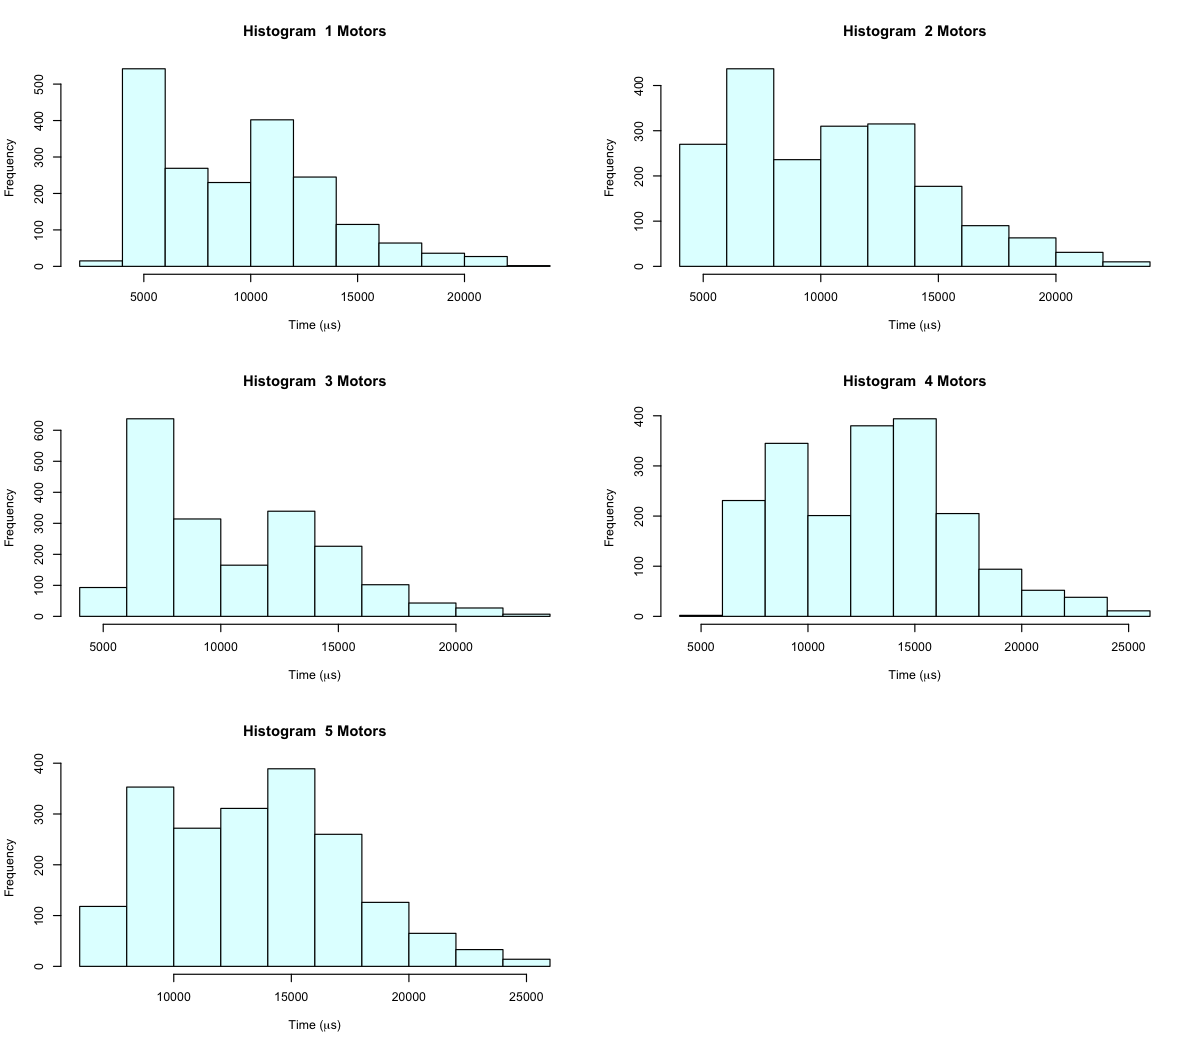
\includegraphics[width=1.0\textwidth]{evaluation/graphics/Xamarin/Galaxy-APITest/HistMotorsXamarinGalaxy-APITest.png}
   \centering
    \caption[Histogramas de motores usando API C\# ]{Histogramas de motores usando API C\# \\Fuente: elaboración propia (2018)} 
    \label{fig:xamarin-galaxy-hist-motors-api}
  \end{center}
\end{figure}

\begin{figure}[H]
  \begin{center} 
   	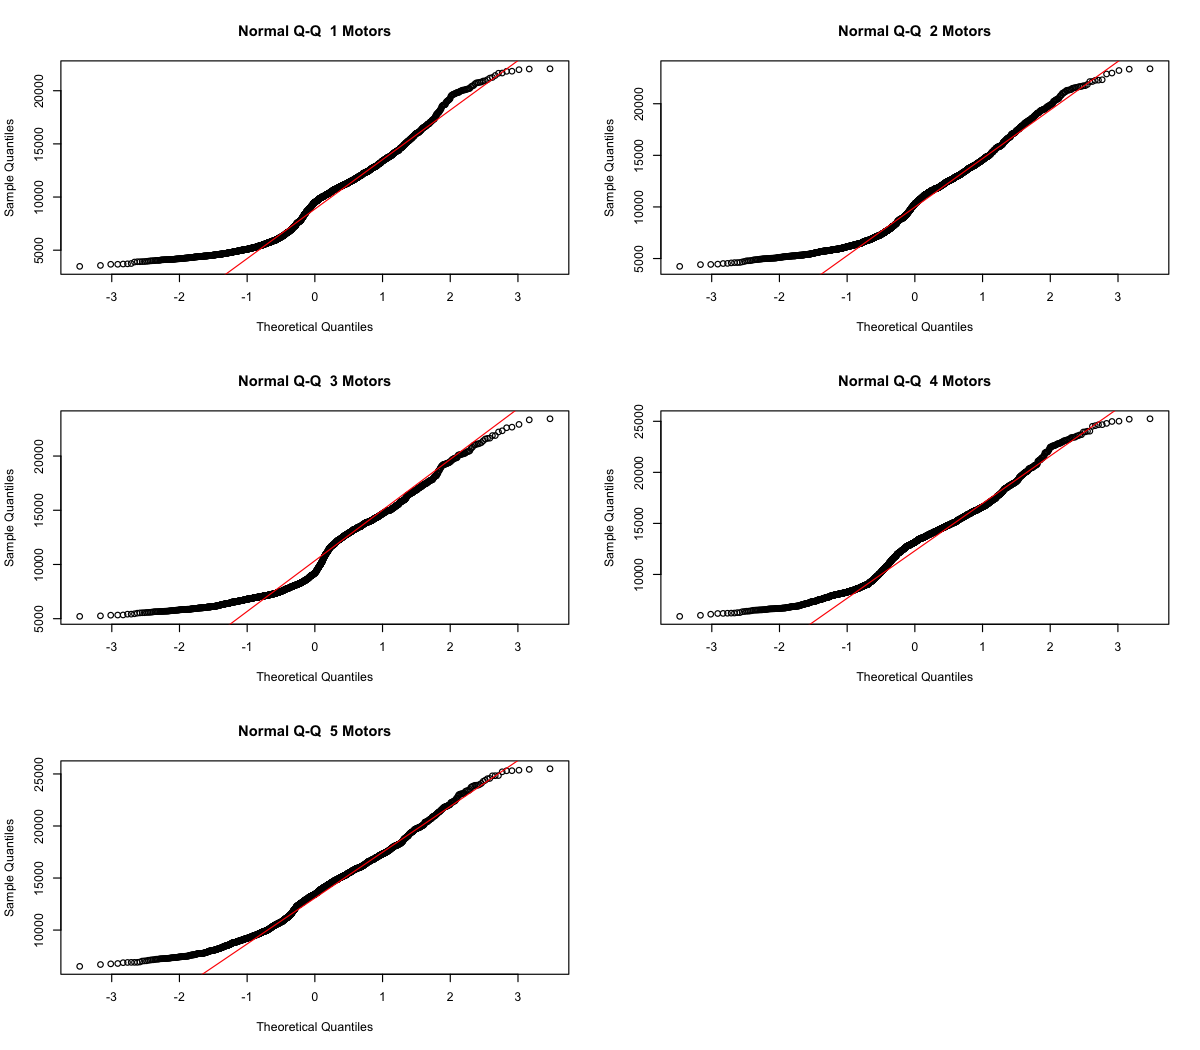
\includegraphics[width=1.0\textwidth]{evaluation/graphics/Xamarin/Galaxy-APITest/NormalQQMotorsXamarinGalaxy-APITest.png} 
   	\centering
    \caption[Gráfico QQ de motores usando API C\# ]{Gráficos QQ de motores usando API C\# \\Fuente: elaboración propia (2018)} 
    \label{fig:xamarin-galaxy-QQ-motors-api}
  \end{center}
\end{figure}

\begin{figure}[H]
  \begin{center} 
   	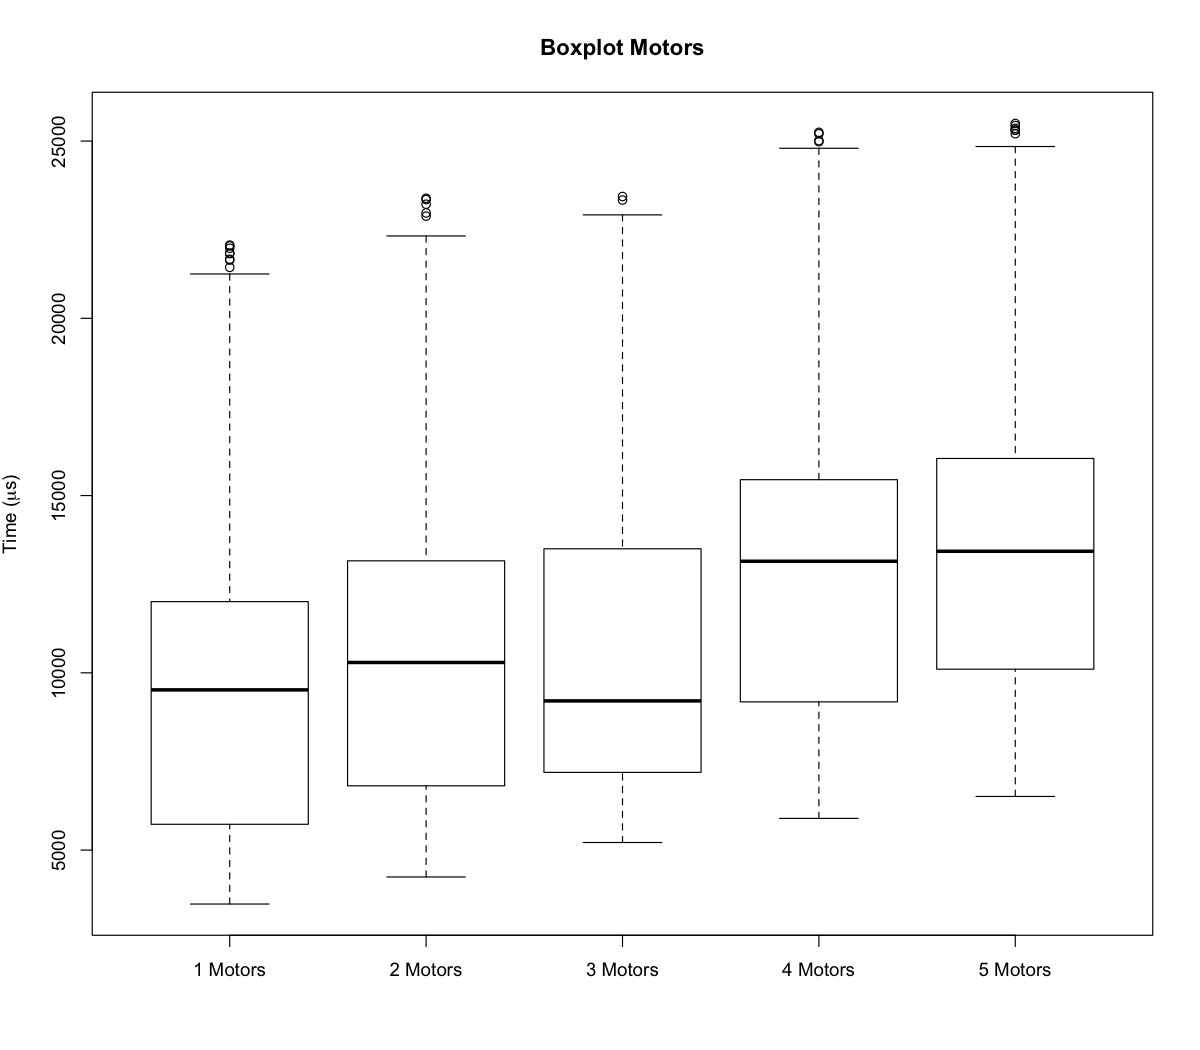
\includegraphics[width=0.8\textwidth]{evaluation/graphics/Xamarin/Galaxy-APITest/BoxplotMotorsXamarinGalaxy-APITest.png} 
   	\centering
    \caption[Gráficos de cajas de motores usando API C\# ]{Gráficos de cajas de motores usando API C\# \\Fuente: elaboración propia (2018)} 
    \label{fig:xamarin-galaxy-boxplot-motors-api}
  \end{center}
\end{figure}

\subsection{API Java}
Para realizar las evaluaciones técnicas de esta API, también fue necesario desarrollar una aplicación nativa en Android, para hacer uso de la API y registrar las latencias obtenidas en las pruebas.